\chapter{Architectural Design}

\section{Overview}
The system will be developed from scratch and it will completely replace the legacy system. \newline

\vspace{0.8em}
\begin{figure}[H]
	\centering
	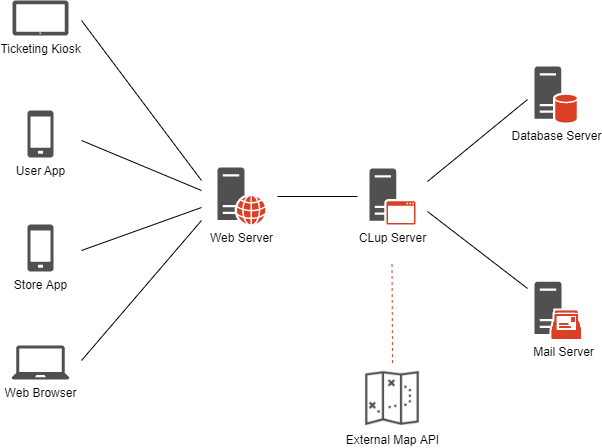
\includegraphics[scale=0.45]{overview_diagram}
	\caption{CLup system diagram.}
\end{figure}


It is composed by a client part and a server part:
\begin{itemize}
	\item \textbf{Server side:}
	\begin{itemize}
		\item \textit{Application Server (CLup Server):} server where all the logic is located. It communicates with other servers and is the central point of the system.
		\item \textit{Web Server:} server used for the communication with the clients.
		\item \textit{Database Server:} server where all data are stored.
		\item \textit{Mail Server:} server used to send confirmation emails about the bookings.
		\item \textit{External map API:} API used to retrieve data about the distance of the user from the store. This information will be used to inform the user of when leave the current place.
	\end{itemize}
	\item \textbf{Client side:}
	\begin{itemize}
		\item \textit{User App:} Application installed on customers smartphone. It allows to retrieve a ticket or book a visit.
		\item \textit{Store App:} Application installed on employees smartphone. It allows to validate store passes.
		\item \textit{Ticketing Kiosk:} Tablet installed at the entrance of the store to which a printer is attached. It has installed a modified version of the mobile app which is able to print the ticket on place.
		\item \textit{Web Browser:} Used by store employees and managers to access the web dashboard.
	\end{itemize}
\end{itemize}

\section{Component view}

\section{Deployment view}

\section{Runtime view}

\section{Component interfaces}

\section{Selected architectural styles and patterns}

\section{Other design decisions}
